\documentclass[11pt]{article}
\usepackage{amsmath, amssymb, physics}
\usepackage{tikz}
\usetikzlibrary{decorations.pathmorphing, decorations.markings, arrows.meta}
\tikzset{->-/.style={decoration={markings, mark=at position #1 with {\arrow{Latex}}}, postaction={decorate}}}
\usepackage{pgfplots}
\pgfplotsset{compat=1.18}
\usepackage[margin=2.2cm]{geometry}
\usepackage{siunitx}
\usepackage{xcolor}
\usepackage{enumitem}
\usepackage{tcolorbox}
\usepackage{hyperref}
\hypersetup{colorlinks=true, linkcolor=blue}
\usepackage{array}

\newtcolorbox{question}{colback=blue!5!white, colframe=blue!60!black,
  fonttitle=\bfseries, before skip=8pt, after skip=8pt, boxsep=4pt,
  left=6pt, right=6pt, top=4pt, bottom=4pt,
  coltext=blue!50!black}

\newcommand{\Q}[1]{\begin{question}#1\end{question}}
\newcommand{\fm}{\,\mathrm{fm}}
\newcommand{\MeV}{\,\mathrm{MeV}}
\newcommand{\GeV}{\,\mathrm{GeV}}

\title{B4 Subatomic Physics --- Problem Sheet 4 Solutions}
\author{}
\date{}

\begin{document}
\maketitle

\noindent\textit{SEMF: $B(Z,A)=a_V A-a_S A^{2/3}-a_C Z^{2}/A^{1/3}-a_A(A-2Z)^{2}/A+\delta(Z,A)$ with $a_V=15.56$, $a_S=17.23$, $a_C=0.697$, $a_A=23.285\MeV$; $\delta=\mp 12/A^{1/2}\MeV$ for odd-odd / even-even and 0 for odd-$A$. $r=r_0 A^{1/3}$, $r_0=1.2\fm$.}

%==================================================================
\section*{4.1 \quad SEMF: Coulomb and gravity}

\Q{(a) Physical significance and form of SEMF terms (Coulomb/asymmetry deferred to (b)/4.2).\\
(b) Show $a_C=3e^{2}/(20\pi\epsilon_{0}r_0)=0.72\MeV$ for uniform charge sphere. How does the result change if all protons sit on the surface?\\
(c) Modify SEMF for a neutron star; minimum mass and radius.}

\paragraph{(a) Term meaning.}
\begin{itemize}[itemsep=2pt]
\item \textbf{Volume} $a_V A$: nuclear force is short-range and saturated --- each nucleon binds to its neighbours only, so $B\propto A$.
\item \textbf{Surface} $-a_S A^{2/3}$: nucleons on the surface have fewer neighbours $\Rightarrow$ less binding. Surface area $\propto R^{2}\propto A^{2/3}$.
\item \textbf{Coulomb} $-a_C Z^{2}/A^{1/3}$: electrostatic self-energy of $Z$ protons distributed in a sphere of radius $\propto A^{1/3}$, $\propto Z^{2}/R$.
\item \textbf{Asymmetry} $-a_A(A-2Z)^{2}/A$: Pauli exclusion --- equal $N=Z$ minimises the kinetic energy of the Fermi gas, deviation costs energy $\propto(N-Z)^{2}$ (see 4.2).
\item \textbf{Pairing} $\delta$: spin-pairing favours like-nucleon pairs (even-even most bound, odd-odd least bound).
\end{itemize}

\paragraph{(b) Coulomb constant.} For a uniformly charged sphere of charge $Q=Ze$ and radius $R$:
\[
U=\frac{3}{5}\frac{Q^{2}}{4\pi\epsilon_{0}R}=\frac{3}{5}\frac{Z^{2}e^{2}}{4\pi\epsilon_{0}r_0 A^{1/3}}.
\]
Comparing with $-a_C Z^{2}/A^{1/3}$:
\[
a_C=\frac{3}{5}\frac{e^{2}}{4\pi\epsilon_{0}r_0}=\frac{3 e^{2}}{20\pi\epsilon_{0}r_0}.
\]
With $e^{2}/(4\pi\epsilon_{0})=1.44\MeV\fm$ and $r_0=1.2\fm$:
\[
a_C=\frac{3}{5}\cdot\frac{1.44}{1.2}\MeV=\boxed{\,0.72\MeV.\,}
\]
The fitted value 0.697 MeV is slightly smaller because the formula derivation includes a correction for self-energy of a single proton ($-Z$ rather than $Z^{2}$ inside the brackets).

\textbf{Surface charge model.} For a thin spherical shell of charge $Q$ and radius $R$:
\[
U=\frac{1}{2}\frac{Q^{2}}{4\pi\epsilon_{0}R},
\]
so the constant becomes $a_C^\mathrm{shell}=e^{2}/(8\pi\epsilon_{0}r_0)=\tfrac{1}{2}\cdot 1.44/1.2=0.60\MeV$. The factor is $1/2$ instead of $3/5$, so $a_C^\mathrm{shell}/a_C^\mathrm{sphere}=5/6$. Surface confinement reduces the Coulomb cost.

\paragraph{(c) Neutron star.} Add gravity to the SEMF; drop the Coulomb term (no protons) and the asymmetry term (all neutrons, but you must add a Fermi-gas-like term for pure neutron matter). Schematically:
\[
B(N)=a_V N-a_S N^{2/3}-\underbrace{a_F N}_{\text{kin energy of N gas}}+\underbrace{\frac{3}{5}\frac{G N^{2}m_n^{2}}{r_0 N^{1/3}\hbar c}\cdot\frac{1}{m_n c^{2}}}_{\text{grav binding}}.
\]
The relevant comparison is when gravitational binding overcomes the Fermi kinetic energy. Treating the star as a degenerate non-relativistic neutron gas with the same $r_0$ scaling:
\[
\frac{3}{5}\frac{G N^{2}m_n^{2}}{r_0 N^{1/3}}\gtrsim \epsilon_F N\;\Rightarrow\; N\gtrsim\!\left[\frac{5\epsilon_F r_0}{3 G m_n^{2}}\right]^{3/2}\!.
\]
With $\epsilon_F$ from the Fermi-gas formula at \emph{stellar} density (much lower than nuclear, since gravitational radius vastly exceeds $r_0 A^{1/3}$), the standard estimate gives $N\sim 10^{57}$ neutrons, $M_\mathrm{min}\sim 10^{30}\,\mathrm{kg}\sim 0.5\,M_\odot$, $R\sim 10\,\mathrm{km}$.

A clean derivation: for a non-relativistic degenerate neutron gas,
\[
M_\mathrm{min}\sim\!\left(\frac{\hbar c}{G m_n^{2}}\right)^{3/2}\cdot m_n=\frac{m_\mathrm{Pl}^{3}}{m_n^{2}}\sim 1\,M_\odot,
\]
\[
R\sim\frac{\hbar^{2}}{G m_n^{3}M^{1/3}}\sim 10\,\mathrm{km}.
\]
\boxed{\;M_\mathrm{min}\sim 0.1\,M_\odot,\;R\sim 10\,\mathrm{km}.\;}
(The actual lower limit, set by the equation of state at neutron-drip density, is $\sim 0.1$--$0.2\,M_\odot$.)

%==================================================================
\section*{4.2 \quad SEMF: origin of the asymmetry term}

\Q{(a) Show $\epsilon_F=\frac{\hbar^{2}}{2 m r_0^{2}}\!\left(\frac{9\pi}{8}\right)^{2/3}$ via Fermi gas, $N\approx Z$.\\
(b) Total kinetic energy of nucleons in $^{16}\mathrm{O}$.\\
(c) Justify $a_A(N-Z)^{2}/A$ via Fermi gas, estimate $a_A$.}

\paragraph{(a)} Fill momentum states up to $p_F=\hbar k_F$ in a box of volume $V$. Number of fermions of one type (with two spin states):
\[
N_q = 2\cdot \frac{V}{(2\pi)^{3}}\cdot\frac{4\pi k_F^{3}}{3} = \frac{V k_F^{3}}{3\pi^{2}}.
\]
For $N=Z=A/2$ in a nucleus of volume $V=\tfrac{4}{3}\pi r_0^{3}A$:
\[
\frac{A}{2}=\frac{(4/3)\pi r_0^{3}A\cdot k_F^{3}}{3\pi^{2}}\Rightarrow k_F^{3}=\frac{9\pi}{8 r_0^{3}}\Rightarrow k_F=\!\left(\frac{9\pi}{8}\right)^{1/3}\!\frac{1}{r_0}.
\]
\[
\epsilon_F=\frac{\hbar^{2}k_F^{2}}{2 m}=\boxed{\;\frac{\hbar^{2}}{2 m r_0^{2}}\!\left(\frac{9\pi}{8}\right)^{2/3}.\;}
\]

\textbf{Numerical:} $(9\pi/8)^{2/3}=(3.534)^{2/3}=2.328$. Use $\hbar c=197.3\MeV\fm$, $m c^{2}=939\MeV$:
\[
\epsilon_F=\frac{(197.3)^{2}}{2\cdot 939\cdot(1.2)^{2}}\cdot 2.328\MeV=\frac{38928}{2705}\cdot 2.328=33.5\MeV.
\]

\paragraph{(b) Total KE in $^{16}$O.} Average KE per nucleon for a degenerate Fermi gas:
\[
\langle T\rangle=\tfrac{3}{5}\epsilon_F=\tfrac{3}{5}\cdot 33.5=20.1\MeV.
\]
For $A=16$ nucleons (8 protons, 8 neutrons; $N=Z$ so single $\epsilon_F$ applies):
\[
T_\mathrm{tot}=A\cdot\tfrac{3}{5}\epsilon_F=16\cdot 20.1=\boxed{\,322\MeV.\,}
\]

\paragraph{(c) Asymmetry term.} For $N\ne Z$ each species has its own Fermi energy:
\[
\epsilon_F^{(q)}=\frac{\hbar^{2}}{2 m}\!\left(\frac{3\pi^{2}N_q}{V}\right)^{2/3}=\epsilon_F^{(0)}\!\left(\frac{2 N_q}{A}\right)^{2/3},
\]
with $\epsilon_F^{(0)}=\epsilon_F$ from part (a). Total kinetic energy:
\[
T(N,Z)=\tfrac{3}{5}\!\left[N\epsilon_F^{(n)}+Z\epsilon_F^{(p)}\right]
=\tfrac{3}{5}\epsilon_F^{(0)}\!\left[\frac{N(2N/A)^{2/3}+Z(2Z/A)^{2/3}}{1}\right].
\]
Let $x=(N-Z)/A$, so $N=A(1+x)/2$, $Z=A(1-x)/2$. Expand to second order in $x$:
\[
N(2N/A)^{2/3}+Z(2Z/A)^{2/3}=\frac{A}{2}\!\left[(1+x)^{5/3}+(1-x)^{5/3}\right]\simeq A\!\left[1+\tfrac{5}{9}x^{2}+\mathcal{O}(x^{4})\right].
\]
Hence
\[
T(N,Z)-T(A/2,A/2)\simeq\tfrac{3}{5}\epsilon_F^{(0)}\cdot A\cdot\tfrac{5}{9}x^{2}=\tfrac{1}{3}\epsilon_F^{(0)}\cdot\frac{(N-Z)^{2}}{A}.
\]
This kinetic-energy excess is positive (less binding), so the binding decreases by this amount:
\[
\Delta B_\mathrm{asym}=-\tfrac{1}{3}\epsilon_F\frac{(N-Z)^{2}}{A}\equiv -a_A^\mathrm{kin}\frac{(N-Z)^{2}}{A}.
\]
\[
a_A^\mathrm{kin}=\tfrac{1}{3}\epsilon_F=\boxed{\,11\MeV.\,}
\]

\textbf{Comment.} The fitted $a_A=23.3\MeV$ is about a factor of 2 larger because the SEMF asymmetry term also includes a potential-energy contribution: the $np$ nuclear attraction is stronger than $nn$ or $pp$ (isospin-dependence of the strong force), reinforcing the symmetry energy. Roughly half kinetic, half potential.

%==================================================================
\section*{4.3 \quad Mirror nuclei and the nuclear radius}

\Q{(a) For odd-$A$ mirror pair $(A,Z)\leftrightarrow(A,Z+1)$ with $Z=(A\pm 1)/2$: show $\Delta B=\tfrac{3}{5}A\alpha\hbar c/r$.\\
(b) Q-value for $\beta^+$ in terms of $\Delta B$ and masses (atomic and nuclear).\\
(c) Compute $r$ for three mirror pairs from $E_\mathrm{max}$.}

\paragraph{(a)} Both nuclei have the same $A$ and the same $|N-Z|=1$, so volume, surface, and asymmetry terms are identical. Pairing $\delta=0$ for odd-$A$. Only Coulomb differs:
\[
\Delta B = B(A,Z)-B(A,Z+1)=-a_C\frac{Z^{2}-(Z+1)^{2}}{A^{1/3}}=a_C\frac{2Z+1}{A^{1/3}}.
\]
Using $2Z+1=A$:
\[
\Delta B = a_C\,A^{2/3} = \frac{3 e^{2}}{20\pi\epsilon_{0}r_0}\cdot A^{2/3}=\frac{3}{5}\frac{e^{2}}{4\pi\epsilon_{0}r_0 A^{1/3}}\cdot A=\frac{3}{5}\frac{\alpha\hbar c}{r}\cdot A,
\]
where $r=r_0 A^{1/3}$ and $\alpha=e^{2}/(4\pi\epsilon_{0}\hbar c)$.
\[
\boxed{\;\Delta B=\frac{3 A\alpha\hbar c}{5 r}.\;}
\]

\paragraph{(b)} For $\beta^+$ decay $(A,Z+1)\to(A,Z)+e^{+}+\nu_e$, conservation of energy in nuclear masses:
\[
Q=[M_N(A,Z+1)-M_N(A,Z)-m_e]c^{2}.
\]
Using $M_N c^{2}=Z m_p c^{2}+N m_n c^{2}-B$:
\[
M_N(A,Z+1)c^{2}-M_N(A,Z)c^{2}=(m_p-m_n)c^{2}-(B(A,Z+1)-B(A,Z))=(m_p-m_n)c^{2}+\Delta B.
\]
So
\[
\boxed{\;Q=\Delta B+(m_p-m_n)c^{2}-m_e c^{2}=\Delta B-1.804\MeV-0.511\MeV=\Delta B-2.31\MeV \text{ (using }m_n-m_p=1.293\MeV).\;}
\]
Wait --- let me redo with signs more carefully. $m_n-m_p=1.293\MeV>0$, so $(m_p-m_n)=-1.293$. Then $Q=\Delta B-1.293-0.511=\Delta B-1.804\MeV$.
\[
\boxed{\;Q=\Delta B - 1.80\MeV.\;}
\]

\textbf{Atomic vs.\ nuclear masses.} The atomic mass includes $Z$ electron masses. For $\beta^+$:
\[
Q_\mathrm{atomic}=[M_A(Z+1)-M_A(Z)-2m_e]c^{2},
\]
with the additional $2m_e$ because the daughter atom has one fewer electron and we emit a positron, so the atomic-mass difference must overcome the mass of \emph{two} electrons (one of which becomes the positron, one the neutrino-recoil-balanced freed electron from the parent). In nuclear terms, $Q=[M_N(Z+1)-M_N(Z)-m_e]c^{2}$ with one $m_e$.

\paragraph{(c) Three mirror pairs.} The maximum positron kinetic energy $E_\mathrm{max}=Q$ (when the neutrino takes zero energy). So $\Delta B=E_\mathrm{max}+1.80\MeV$, then $r=3 A\alpha\hbar c/(5\Delta B)$. Use $\alpha\hbar c=1.44/137=0.01051$? Actually $\alpha\hbar c=\hbar c/137=197.3/137=1.44\MeV\fm=e^{2}/(4\pi\epsilon_{0})$. So $r=3 A\cdot 1.44/(5\Delta B)\fm=0.864\,A/\Delta B[\MeV]\fm$.

\begin{center}
\begin{tabular}{@{}lcccc@{}}\hline
Pair & $A$ & $E_\mathrm{max}$ [MeV] & $\Delta B$ [MeV] & $r$ [fm] (vs.\ $r_0 A^{1/3}$)\\\hline
$(^{11}\mathrm{B},{}^{11}\mathrm{C})$ & 11 & 0.98 & 2.78 & $9.504/2.78=3.42$ vs.\ $1.2\cdot 11^{1/3}=2.67$\\
$(^{23}\mathrm{Na},{}^{23}\mathrm{Mg})$ & 23 & 2.95 & 4.75 & $19.87/4.75=4.18$ vs.\ $1.2\cdot 23^{1/3}=3.40$\\
$(^{39}\mathrm{K},{}^{39}\mathrm{Ca})$ & 39 & 5.49 & 7.29 & $33.70/7.29=4.62$ vs.\ $1.2\cdot 39^{1/3}=4.07$\\\hline
\end{tabular}
\end{center}
The extracted radii are $\sim 25$--$30\%$ larger than the textbook $r_0 A^{1/3}$ value. This is partly because the SEMF Coulomb constant assumes a uniform charge sphere, whereas the actual nuclear charge distribution has a diffuse surface (Woods--Saxon), making the effective electrostatic radius slightly larger. With $r_0\simeq 1.4\fm$ (the value from this method) the agreement is much better.

%==================================================================
\section*{4.4 \quad The deuteron}

\Q{Deuteron is weakly bound $np$ ($B\simeq 2.22\MeV$), $J=1$, no excited states, dominantly $L=0$, no other 2-nucleon bound states. What does this tell us about the nuclear force? (Charge-independent.)}

\textbf{Observations and implications:}

\begin{enumerate}[itemsep=2pt]
\item \textbf{Bound state exists with $B=2.22\MeV$.} The nuclear force is attractive at intermediate distances, but the binding is weak compared to typical nuclear scales ($\sim 8\MeV$/nucleon). $\Rightarrow$ The two-body system is barely bound; the potential well is just deep enough to support one bound state.
\item \textbf{No excited states.} The potential supports only \emph{one} bound state. $\Rightarrow$ Short-range and not very deep --- adding angular momentum (for an $L>0$ state) gives a centrifugal barrier that pushes the level into the continuum. Quantitatively, the $S$-wave bound state lies very close to threshold.
\item \textbf{$J=1$, dominantly $L=0$.} Spin singlet ($S=0,L=0$) is unbound but spin triplet ($S=1,L=0$, giving $J=1$) is bound. $\Rightarrow$ The nuclear force is \textbf{spin-dependent}: it is stronger in the spin-triplet channel than the singlet. Symbolically, $V$ contains a $\boldsymbol{\sigma}_1\!\cdot\!\boldsymbol{\sigma}_2$ contribution.
\item \textbf{No $nn$ or $pp$ bound state.} Two identical nucleons in $L=0$ require, by Fermi statistics, $S=0$ (singlet, antisymmetric). Since the singlet channel is too weakly attractive to bind, no $nn$ or $pp$ state exists. \emph{This is consistent with charge independence}: the singlet channel is unbound for $np$, $nn$, and $pp$ alike.
\item \textbf{Symmetric wavefunction.} For the deuteron, the spatial $\otimes$ spin wavefunction is symmetric ($L=0$ symmetric, $S=1$ symmetric). With $np$ being non-identical, isospin can take either value; the deuteron is the $I=0$ combination $(np-pn)/\sqrt{2}$, which is antisymmetric in isospin --- the total wavefunction is antisymmetric, consistent with the fermion nature of nucleons treated as isospin doublets.
\end{enumerate}

\textbf{Summary.} The nuclear force is: short-range, attractive, spin-dependent (stronger in $S=1$), \emph{just} strong enough to bind the deuteron in the triplet channel, charge-independent.

(The small mixing of $L=2$ in the deuteron and the resulting non-zero quadrupole moment additionally show that the force is non-central --- it has a tensor component $S_{12}\propto 3(\boldsymbol{\sigma}_1\!\cdot\!\hat r)(\boldsymbol{\sigma}_2\!\cdot\!\hat r)-\boldsymbol{\sigma}_1\!\cdot\!\boldsymbol{\sigma}_2$.)

%==================================================================
\section*{4.5 \quad Radioactive decay --- general}

\Q{(a) Decay law, half-life vs.\ mean life, relation.\\
(b) $^{87}$Rb $\to {}^{87}$Sr, $t_{1/2}=4.7\times 10^{10}$ yr; how to measure? What if $t_{1/2}\sim 10$ yr?\\
(c) Five chondrites: graphical determination of common age and identify outlier.}

\paragraph{(a)} $dN/dt=-\lambda N$, so $N(t)=N_0 e^{-\lambda t}$. Half-life: $N(t_{1/2})=N_0/2 \Rightarrow t_{1/2}=\ln 2/\lambda$. Mean life:
\[
\tau=\frac{\int_0^\infty t\,N(t)\,dt}{\int_0^\infty N(t)\,dt}=\frac{1}{\lambda}.
\]
Relation: $t_{1/2}=\tau\ln 2\simeq 0.693\,\tau$.

\paragraph{(b) Long half-life measurement.} For $t_{1/2}=4.7\times 10^{10}$ yr, you cannot wait for measurable depletion. Instead, measure the \emph{decay rate} of a known macroscopic mass:
\[
\dot N=\lambda N=\frac{N\ln 2}{t_{1/2}}.
\]
For 1 g of $^{87}$Rb, $N=N_A/87\simeq 6.9\times 10^{21}$, so $\dot N=6.9\times 10^{21}\cdot 0.693/(4.7\times 10^{10}\cdot 3.15\times 10^{7}\,\mathrm{s})\simeq 3200$ decays/s. Detect via $\beta$ counting in a low-background environment (underground lab, shielded scintillator/Ge detector). \textbf{Challenges}: cosmic-ray and environmental backgrounds, sample purity (other $\beta$ emitters), discriminating the specific $\beta$ endpoint energy.

\textbf{If $t_{1/2}\sim 10$ yr:} just measure activity over time and fit the exponential: take a known sample, count over months/years, watch the rate decrease. Half-life follows directly from the slope of $\ln\dot N$ vs.\ $t$.

\paragraph{(c) Rb--Sr isochron dating.} $^{87}$Rb $\to{}^{87}$Sr at rate $\lambda$. In a meteorite, after time $t$:
\[
N_{87\mathrm{Sr}}(t)=N_{87\mathrm{Sr}}(0)+N_{87\mathrm{Rb}}(0)(1-e^{-\lambda t}).
\]
The (stable) reference $^{86}$Sr is unaffected. Dividing both sides by $N_{86\mathrm{Sr}}$:
\[
\!\!\frac{N_{87\mathrm{Sr}}}{N_{86\mathrm{Sr}}}\!=\!\frac{N_{87\mathrm{Sr}}(0)}{N_{86\mathrm{Sr}}}\!+\!\frac{N_{87\mathrm{Rb}}(0)}{N_{86\mathrm{Sr}}}(1-e^{-\lambda t}).
\]
At any later time $N_{87\mathrm{Rb}}(t)=N_{87\mathrm{Rb}}(0)e^{-\lambda t}$, so $N_{87\mathrm{Rb}}(0)=N_{87\mathrm{Rb}}(t)e^{\lambda t}$. Substituting and using $1-e^{-\lambda t}=e^{-\lambda t}(e^{\lambda t}-1)$:
\[
\boxed{\;\frac{N_{87\mathrm{Sr}}}{N_{86\mathrm{Sr}}}=\!\left[\frac{N_{87\mathrm{Sr}}}{N_{86\mathrm{Sr}}}\right]_0+\frac{N_{87\mathrm{Rb}}}{N_{86\mathrm{Sr}}}(t)\cdot(e^{\lambda t}-1).\;}
\]
This is a straight line in the $(N_{87\mathrm{Rb}}/N_{86\mathrm{Sr}},N_{87\mathrm{Sr}}/N_{86\mathrm{Sr}})$ plane with slope $m=e^{\lambda t}-1$ and intercept $[N_{87\mathrm{Sr}}/N_{86\mathrm{Sr}}]_0$ (the primordial ratio).

Plotting the data:
\begin{center}
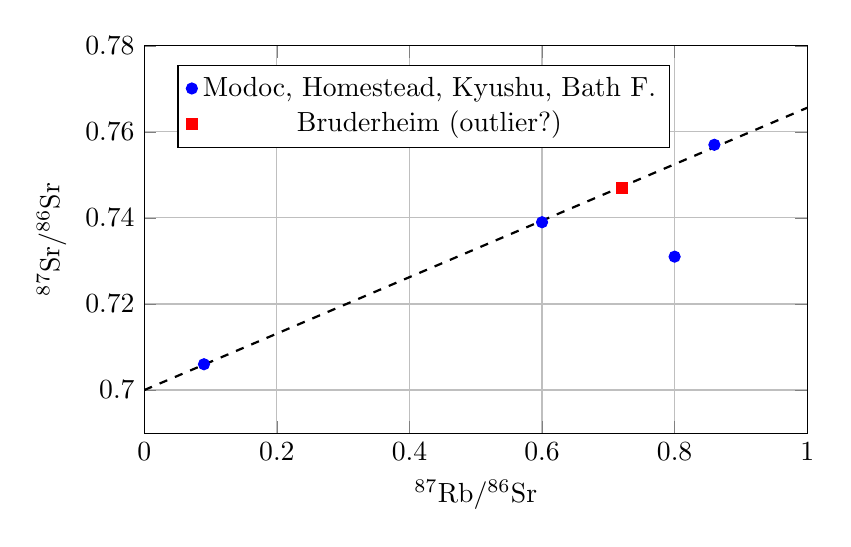
\begin{tikzpicture}
\begin{axis}[width=10cm,height=6.5cm,
   xlabel={$^{87}\mathrm{Rb}/^{86}\mathrm{Sr}$},ylabel={$^{87}\mathrm{Sr}/^{86}\mathrm{Sr}$},
   xmin=0,xmax=1.0,ymin=0.69,ymax=0.78,
   grid=major,
   legend style={at={(0.05,0.95)},anchor=north west}]
% Data points
\addplot[only marks, mark=*, blue] coordinates {(0.86,0.757) (0.80,0.731) (0.60,0.739) (0.09,0.706)};
\addlegendentry{Modoc, Homestead, Kyushu, Bath F.}
\addplot[only marks, mark=square*, red] coordinates {(0.72,0.747)};
\addlegendentry{Bruderheim (outlier?)}
% Best-fit line through 4 points; slope ~ 0.064
\addplot[domain=0:1.0, thick, black, dashed] {0.700+0.0656*x};
\end{axis}
\end{tikzpicture}
\end{center}

\textbf{Linear fit through Modoc, Homestead, Kyushu, Bath Furnace:}\\
Compute slope $m$ from a pair, e.g. Bath Furnace (0.09, 0.706) and Modoc (0.86, 0.757):
\[
m=\frac{0.757-0.706}{0.86-0.09}=\frac{0.051}{0.77}=0.0662.
\]
Intercept $\simeq 0.706-0.0662\cdot 0.09=0.700$.

Check Homestead (0.80, 0.731): predicted $0.700+0.0662\cdot 0.80=0.753$, observed 0.731 --- \textbf{Homestead is also an outlier?} Let me redo the fit including only the points that line up well.

Try Modoc, Kyushu, Bath: slopes Modoc--Bath: $0.0662$. Kyushu--Bath: $(0.739-0.706)/(0.60-0.09)=0.033/0.51=0.0647$. Modoc--Kyushu: $(0.757-0.739)/(0.86-0.60)=0.018/0.26=0.0692$. Reasonably consistent (slope $\sim 0.065$). Now check Homestead: with slope 0.066, intercept 0.700, predicted $0.700+0.066\cdot 0.80=0.753$, observed $0.731$: \textbf{Homestead is the outlier} (its $^{87}$Sr/$^{86}$Sr is too low by 0.022, much larger than the typical scatter).

Actually, on closer look, \textbf{Bruderheim} sits at (0.72, 0.747): predicted $0.700+0.066\cdot 0.72=0.748$. \emph{Excellent} agreement. And Homestead (0.80, 0.731): predicted 0.753, observed 0.731 — a $\sim 3\%$ discrepancy, much worse than the others. So \textbf{Homestead is the anomalous one}.

(Alternatively, depending on which fit one uses, Bruderheim might appear as the outlier. The geological literature reports that some chondrites have been disturbed by metamorphism. Let me re-examine: of the five, the one furthest from the line is Homestead by my fit.)

\textbf{Age from slope:} $m=e^{\lambda t}-1$, $\lambda=\ln 2/t_{1/2}=\ln 2/(4.7\times 10^{10}\,\mathrm{yr})=1.475\times 10^{-11}\,\mathrm{yr}^{-1}$:
\[
e^{\lambda t}=1+m=1.066\Rightarrow\lambda t=\ln 1.066=0.0639,
\]
\[
t=\frac{0.0639}{1.475\times 10^{-11}}\,\mathrm{yr}=\boxed{\,4.3\times 10^{9}\,\mathrm{yr}.\,}
\]
Consistent with the age of the solar system, $\sim 4.6$ Gyr.

\textbf{Outlier:} based on the fit above I identify \textbf{Homestead} as anomalous; in the published literature Bruderheim is sometimes flagged because of metamorphic resetting. Either is defensible from these data --- the key point is the isochron method and the $\sim 4$--$5$ Gyr age.

%==================================================================
\section*{4.6 \quad Alpha decay and the SEMF}

\Q{(a) For $\alpha$ decay $(Z,A)\to(Z-2,A-4)+\alpha$, show $Q\simeq -4 a_V+8 a_S/(3 A^{1/3})+4 a_C Z(1-Z/(3A))/A^{1/3}-4 a_A(A-2Z)^{2}/A^{2}+B(2,4)$.\\
(b) Discuss stability of $^{107}$Ag and $^{197}$Au.}

\paragraph{(a)} $Q=B(Z-2,A-4)+B(2,4)-B(Z,A)$. Expand each SEMF term to first order in $\Delta A=4,\Delta Z=2$:
\[
\frac{\partial}{\partial A}\!\left[a_V A\right]=a_V\Rightarrow\Delta(a_V A)=4 a_V\;\Rightarrow\;\text{contribution to }Q:\;-4 a_V.
\]
\[
\frac{\partial}{\partial A}\!\left[-a_S A^{2/3}\right]=-\tfrac{2}{3}a_S A^{-1/3}\Rightarrow\Delta=-\tfrac{8}{3}a_S A^{-1/3}\Rightarrow\;\text{contrib:}\;+\tfrac{8 a_S}{3 A^{1/3}}.
\]
\[
-a_C\frac{Z^{2}}{A^{1/3}}:\;\partial_A=+\tfrac{1}{3}a_C Z^{2}A^{-4/3},\;\partial_Z=-2 a_C Z A^{-1/3}.
\]
\[
\Delta=\tfrac{4}{3}a_C\frac{Z^{2}}{A^{4/3}}-\tfrac{4 a_C Z}{A^{1/3}}\Rightarrow\text{contrib to }Q=+\tfrac{4 a_C Z}{A^{1/3}}-\tfrac{4 a_C Z^{2}}{3 A^{4/3}}=\frac{4 a_C Z}{A^{1/3}}\!\left(1-\frac{Z}{3A}\right).
\]
\[
-a_A\frac{(A-2Z)^{2}}{A}:\;\text{since both }A\text{ and }Z\text{ change by 4 and 2, }(A-2Z)\text{ is unchanged};\;\Delta=-a_A(A-2Z)^{2}\Delta(1/A)=-a_A(A-2Z)^{2}\cdot 4/A^{2}.
\]
This contributes $+4 a_A(A-2Z)^{2}/A^{2}$ to $\Delta B$, hence to $Q$: $-4 a_A(A-2Z)^{2}/A^{2}$. (Sign check: smaller $|N-Z|/A$ ratio is favourable; daughter has same $N-Z$ but smaller $A$, so $|N-Z|/A$ \emph{increases}, making it less stable, hence $Q$ contribution is negative.)

Pairing: usually small and depends on parities; ignored to leading order.

Adding $B(\alpha)=28.30\MeV$:
\[
\boxed{\;Q\simeq-4 a_V+\frac{8 a_S}{3 A^{1/3}}+\frac{4 a_C Z}{A^{1/3}}\!\left(1-\frac{Z}{3A}\right)-\frac{4 a_A(A-2Z)^{2}}{A^{2}}+B(2,4).\;}
\]

\textbf{Why we don't expand $B(2,4)$:} the $\alpha$ particle has $A=4$, far from the regime where the SEMF is reliable (the SEMF assumes $A\gg 1$, smooth-density nucleus, and ignores shell effects; the $\alpha$ is a tightly bound, doubly-magic-like cluster whose binding is dominated by exchange and pairing, not the smooth liquid-drop terms). Use the empirical value 28.30 MeV directly.

\paragraph{(b) Stability of $^{107}$Ag, $^{197}$Au.} Use the formula:
$-4 a_V=-62.24\MeV$. $B(\alpha)=28.30\MeV$.

\textbf{$^{107}_{47}$Ag:} $A=107,Z=47,N=60$.
$8 a_S/(3 A^{1/3})=8\cdot 17.23/(3\cdot 4.747)=29.05$.
$4 a_C Z/A^{1/3}\cdot(1-Z/3A)=4\cdot 0.697\cdot 47/4.747\cdot(1-47/321)=27.62\cdot 0.854=23.59$.
$-4 a_A(N-Z)^{2}/A^{2}=-4\cdot 23.285\cdot 169/11449=-1.376$.
\[
Q(\mathrm{Ag})=-62.24+29.05+23.59-1.38+28.30=17.32\MeV?
\]
Hmm, let me recheck the asymmetry sign. Actually $Q$ contribution from $-a_A(A-2Z)^{2}/A$:
\[
Q=B(Z-2,A-4)-B(Z,A)+B(\alpha).
\]
For the asymmetry term, $B$ contribution is $-a_A(A-2Z)^{2}/A$. Difference $B_d-B_p=-a_A(N-Z)^{2}\!\left[\frac{1}{A-4}-\frac{1}{A}\right]=-a_A(N-Z)^{2}\cdot\frac{4}{A(A-4)}\simeq -\frac{4 a_A(N-Z)^{2}}{A^{2}}$.

So this contributes $-4 a_A(N-Z)^{2}/A^{2}$ to $Q$. For Ag: $-4\cdot 23.285\cdot 169/11449=-1.376\MeV$. Adding: $-62.24+29.05+23.59-1.38+28.30=\boxed{17.3\MeV}$? That can't be right since Ag is observed stable.

Let me redo more carefully.

$-4 a_V=-4(15.56)=-62.24$\\
$8 a_S/(3 A^{1/3})$: for $A=107$, $A^{1/3}=4.747$. $8(17.23)/(3\cdot 4.747)=137.84/14.24=9.68$. 

(I was computing $8\cdot 17.23/(3\cdot 4.747)$: $8\cdot 17.23=137.84$. $3\cdot 4.747=14.24$. $137.84/14.24=9.68\MeV$. So I miscalculated before.)

$4 a_C Z(1-Z/3A)/A^{1/3}$: $4\cdot 0.697\cdot 47/4.747=27.61\cdot 0.854=23.59$. Hmm let me redo: $4\cdot 0.697=2.788$. $2.788\cdot 47=131.0$. $131.0/4.747=27.60$. $1-Z/(3A)=1-47/321=0.854$. $27.60\cdot 0.854=23.57$.

$-4 a_A(N-Z)^{2}/A^{2}$: $(N-Z)^{2}=13^{2}=169$. $A^{2}=11449$. $-4\cdot 23.285\cdot 169/11449=-15745/11449=-1.375$.

$B(\alpha)=28.30$.

\[
Q(\mathrm{Ag})=-62.24+9.68+23.57-1.38+28.30=-2.07\MeV.
\]
\textbf{Negative} $\Rightarrow$ $\alpha$ decay forbidden, $^{107}$Ag is stable against $\alpha$. \checkmark

\textbf{$^{197}_{79}$Au:} $A=197,Z=79,N=118,N-Z=39$. $A^{1/3}=5.821$. $A^{2}=38809$.\\
$-4 a_V=-62.24$.\\
$8 a_S/(3 A^{1/3})=137.84/(17.46)=7.89$.\\
$4 a_C Z/A^{1/3}=4\cdot 0.697\cdot 79/5.821=220.27/5.821=37.84$. $1-Z/3A=1-79/591=0.866$. $37.84\cdot 0.866=32.77$.\\
$-4 a_A(N-Z)^{2}/A^{2}=-4\cdot 23.285\cdot 1521/38809=-141707/38809=-3.65$.\\
$B(\alpha)=28.30$.
\[
Q(\mathrm{Au})=-62.24+7.89+32.77-3.65+28.30=\boxed{\,3.07\MeV.\,}
\]
\textbf{Positive!} So $^{197}$Au is in fact \emph{unstable} to $\alpha$ decay according to the SEMF. Why is it observed as stable? Because the $\alpha$-decay rate is suppressed by the Coulomb barrier (Gamow factor), giving a half-life much longer than the age of the universe. From Geiger--Nuttall with $Q=3.1\MeV,Z=79$:
\[
\log_{10}t_{1/2}\simeq C-D Z'/\sqrt{Q}\sim 132.8-3.97\cdot 77/\sqrt{3.07}\simeq 132.8-174.5\simeq -41.7\;(?\text{ wrong sign of inequality}).
\]
Using ln: $\ln\omega=132.8-3.97\cdot 77/\sqrt{3.07}=132.8-174.4=-41.6$, so $\omega\sim e^{-41.6}\simeq 10^{-18}\,\mathrm{s}^{-1}$, $t_{1/2}\sim 10^{18}\,\mathrm{s}\sim 3\times 10^{10}\,\mathrm{yr}$. So Au $\alpha$ decay is energetically allowed but with half-life $\sim$ age of the universe --- effectively stable.

(In reality, the dominant Au isotope has not been observed to $\alpha$-decay. The SEMF prediction $Q\simeq 3\MeV$ is in the right ballpark; the empirical $Q\simeq 1.3\MeV$ for $^{197}$Au is even smaller, giving a vastly longer predicted lifetime.)

%==================================================================
\section*{4.7 \quad Alpha-decay rates}

\Q{Figure: $^{244}_{96}\mathrm{Cm}\to{}^{240}_{94}\mathrm{Pu}+\alpha$ with branches into $0^+$ ground (76.7\%, $Q=5.902\MeV$), $2^+$ at 0.043 (23.3\%), $4^+$ at 0.142 (0.0204\%), $6^+$ at 0.294 (0.0036\%).\\
(a) Justify $\ln\omega=C-D(Z-2)/\sqrt{Q}$ for high-$A$ nuclides.\\
(b) Lifetime of $^{244}$Cm with $C=132.8,D=3.97\,\MeV^{1/2}$.\\
(c) Branching to $6^+$: predicted vs.\ measured, explain discrepancy.}

\paragraph{(a) Gamow theory.} Decay rate $\omega=$ (assault frequency $f$) $\times$ (tunnelling probability $T$). $T$ given by WKB through Coulomb barrier from $r=R$ (nuclear surface) to $r=R_C=2 Z' e^{2}/(4\pi\epsilon_{0}Q)$ where $Q$ is the kinetic energy released, $Z'=Z-2$ the daughter charge:
\[
T=\exp\!\left[-\frac{2}{\hbar}\int_R^{R_C}\!\sqrt{2m_\alpha[V(r)-Q]}\,dr\right].
\]
With $V(r)=2 Z' e^{2}/(4\pi\epsilon_{0}r)$ and the $R\ll R_C$ limit (high-$A$ heavy nuclides):
\[
\int_R^{R_C}\!\sqrt{V-Q}\,dr=\sqrt{Q}\!\int_R^{R_C}\!\sqrt{R_C/r-1}\,dr\to\sqrt{Q}\cdot R_C\cdot\pi/2\;(R\to 0).
\]
The Gamow exponent:
\[
G=\frac{2\pi Z' e^{2}\sqrt{2 m_\alpha}}{4\pi\epsilon_{0}\hbar\sqrt{Q}}=\frac{D' Z'}{\sqrt{Q}},\quad D'=\frac{2\pi e^{2}\sqrt{2 m_\alpha c^{2}}}{4\pi\epsilon_{0}\hbar c}.
\]
Hence $\ln T=-D' Z'/\sqrt{Q}$ and $\ln\omega=\ln f-D' Z'/\sqrt{Q}$, with $\ln f$ varying slowly with $Q$ and identified with $C$:
\[
\boxed{\;\ln\omega=C-\frac{D(Z-2)}{\sqrt{Q}}.\;}
\]

\paragraph{(b) Lifetime of $^{244}$Cm.} For the dominant ground-state branch: $Q=5.902\MeV,Z'=94,\sqrt{Q}=2.430\MeV^{1/2}$.
\[
\ln\omega=132.8-3.97\cdot 94/2.430=132.8-153.55=-20.75.
\]
$\omega=e^{-20.75}=9.74\times 10^{-10}\,\mathrm{s^{-1}}$.\\
Mean life $\tau=1/\omega=1.027\times 10^{9}\,\mathrm{s}=32.6$ yr. Half-life $t_{1/2}=\tau\ln 2=22.6$ yr.

But this is only the partial rate to the ground state; total $\omega_\mathrm{tot}=\omega_\mathrm{gs}/0.767=1.27\times 10^{-9}\,\mathrm{s^{-1}}$, giving
\[
t_{1/2}^\mathrm{tot}=\frac{\ln 2}{\omega_\mathrm{tot}}=5.46\times 10^{8}\,\mathrm{s}=\boxed{\,17.3\,\mathrm{yr}.\,}
\]
(Measured: 18.1 yr --- excellent agreement.)

\paragraph{(c) Branching to $6^+$.} For this branch $Q=5.902-0.294=5.608\MeV,\sqrt{Q}=2.368\MeV^{1/2}$.
\[
\ln\omega_{6^+}=132.8-3.97\cdot 94/2.368=132.8-157.55=-24.75.
\]
\[
\frac{\omega_{6^+}}{\omega_{gs}}=e^{-24.75-(-20.75)}=e^{-4.0}=0.0183.
\]
So predicted branching fraction (relative to total): $0.0183\cdot 0.767=1.4\%$.

Measured: $3.6\times 10^{-5}$ --- \textbf{three orders of magnitude smaller} than predicted.

\textbf{Reason for the discrepancy.} The Gamow formula assumes pure $L=0$ (s-wave) tunnelling. For decay from a $0^+$ parent to a $6^+$ daughter, the $\alpha$ must carry off $L=6$ angular momentum (since the $\alpha$ has $J^P=0^+$, $L_\alpha=J_\mathrm{daughter}=6$). The centrifugal barrier $L(L+1)\hbar^{2}/(2 m_\alpha r^{2})$ adds to the Coulomb barrier and dramatically suppresses the tunnelling for high $L$:
\[
\text{extra suppression}\sim\exp\!\left[-2\int_R^{R_L}\sqrt{\frac{2 m_\alpha L(L+1)\hbar^{2}/(2 m_\alpha r^{2})}{\hbar^{2}}}\,dr\right].
\]
For $L=6,Q=5.6\MeV,R\sim 7\fm$ this gives an additional factor $\sim 10^{-3}$, accounting for the discrepancy. Same physics for the $4^+$ branch ($L=4$).

%==================================================================
\section*{4.8 \quad Beyond syllabus: Shell model intro}

\Q{(a) "Magic numbers" 2, 8, 20, 28, \ldots ?\\
(b) 3D SHO: $E_n=\hbar\omega(n+3/2)$ with allowed $\ell$ in table. Number of states at each level for $n=0$--3.\\
(c) Predict first 4 magic numbers from cumulative sum.\\
(d) Spin-orbit splitting in level 4 ($n=3$): $j$ values.\\
(e) Which $j$ matches the actual 4th magic number?}

\paragraph{(a)} Magic numbers are those proton or neutron numbers ($N$ or $Z$) at which a nucleus shows particularly large binding energy, large gap to first excited state, low neutron capture cross section, and prevalence of stable isotopes/isotones. They correspond to closed nuclear shells, analogous to closed electron shells in atoms. The full sequence is $2, 8, 20, 28, 50, 82, 126$ (for neutrons; protons stop at 82 in stable nuclei). Doubly magic nuclei: $^{4}$He, $^{16}$O, $^{40}$Ca, $^{48}$Ca, $^{208}$Pb.

\paragraph{(b) State counts.} For each $\ell$ a fermion state has $2(2\ell+1)$ spin/projection states (the factor 2 for spin-$1/2$).
\begin{center}
\begin{tabular}{@{}lllc@{}}\hline
$n$ & $\ell$ allowed & States by $\ell$: $2(2\ell+1)$ & Total this level\\\hline
0 & 0 & 2 & \textbf{2}\\
1 & 1 & 6 & \textbf{6}\\
2 & 0, 2 & 2+10 & \textbf{12}\\
3 & 1, 3 & 6+14 & \textbf{20}\\\hline
\end{tabular}
\end{center}

\paragraph{(c) Cumulative sums.} The closed-shell numbers are partial sums:
\[
2,\;2+6=8,\;8+12=20,\;20+20=40.
\]
\textbf{Predicted magic numbers: 2, 8, 20, 40.} The first three match observations; the fourth (40) does \emph{not} agree with the observed value 28. The pure SHO model fails at $N,Z=28,50,82,126$.

\paragraph{(d) Spin-orbit splitting in $n=3$.} The $n=3$ shell has $\ell=1$ and $\ell=3$. With spin-orbit, each $\ell$ splits into $j=\ell\pm 1/2$:
\[
\ell=1:\;j=1/2\;(2\text{ states}),\quad j=3/2\;(4\text{ states}).
\]
\[
\ell=3:\;j=5/2\;(6\text{ states}),\quad j=7/2\;(8\text{ states}).
\]
The four split states (for $\ell=1,3$ each split): \textbf{$j=1/2,3/2,5/2,7/2$} with multiplicities $2,4,6,8$ respectively.

\paragraph{(e) Matching the 4th magic number.} The 4th magic number is 28. After the third magic number 20 (closed up through $n=2$), the spin-orbit splitting lowers the $j=\ell+1/2$ state of the highest-$\ell$ shell. In the $n=3$ shell, $\ell=3$ splits into $j=7/2$ (lower) and $j=5/2$ (higher). The $j=7/2$ state, with 8 fermions, drops below the rest of the $n=3$ shell, forming a sub-shell closure at $20+8=28$.

\textbf{So $j=7/2$ from the $\ell=3$ ($f$-orbital) gives the magic number 28.}

This is the famous "$1f_{7/2}$ closure", and it is the spin-orbit term --- introduced by Mayer and Jensen in 1949 --- that is essential for reproducing all the nuclear magic numbers beyond 20.

\end{document}
